

\tikzset{every picture/.style={line width=1pt}} %set default line width to 0.75pt        

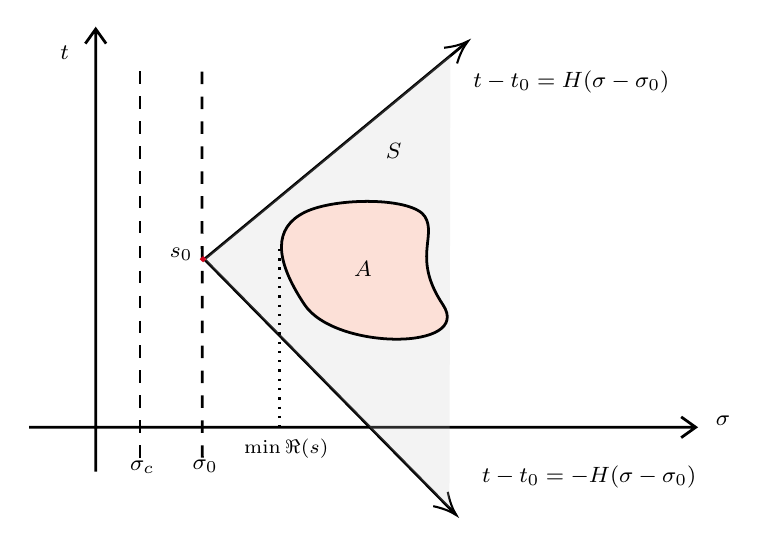
\begin{tikzpicture}[x=0.75pt,y=0.75pt,yscale=-1,xscale=1]
%uncomment if require: \path (0,300); %set diagram left start at 0, and has height of 300

%Shape: Axis 2D [id:dp1346371884561901] 
\draw  (126.5,222.43) -- (447.69,222.43)(158.62,30.58) -- (158.62,243.75) (440.69,217.43) -- (447.69,222.43) -- (440.69,227.43) (153.62,37.58) -- (158.62,30.58) -- (163.62,37.58)  ;
%Straight Lines [id:da6627378326231086] 
\draw  [dash pattern={on 4.5pt off 4.5pt}]  (209.79,51.11) -- (210,238.5) ;
%Straight Lines [id:da15935893462766404] 
\draw    (210.34,140.83) -- (331,263.37) ;
\draw [shift={(332.4,264.8)}, rotate = 225.45] [color={rgb, 255:red, 0; green, 0; blue, 0 }  ][line width=0.75]    (10.93,-4.9) .. controls (6.95,-2.3) and (3.31,-0.67) .. (0,0) .. controls (3.31,0.67) and (6.95,2.3) .. (10.93,4.9)   ;
%Straight Lines [id:da1539498165538844] 
\draw    (211,141.43) -- (336.46,37.67) ;
\draw [shift={(338,36.4)}, rotate = 140.41] [color={rgb, 255:red, 0; green, 0; blue, 0 }  ][line width=0.75]    (10.93,-4.9) .. controls (6.95,-2.3) and (3.31,-0.67) .. (0,0) .. controls (3.31,0.67) and (6.95,2.3) .. (10.93,4.9)   ;
%Shape: Ellipse [id:dp5156478132048201] 
\draw  [color={rgb, 255:red, 208; green, 2; blue, 27 }  ,draw opacity=1 ][fill={rgb, 255:red, 208; green, 2; blue, 27 }  ,fill opacity=1 ] (209.69,141.43) .. controls (209.69,141.1) and (209.98,140.83) .. (210.34,140.83) .. controls (210.71,140.83) and (211,141.1) .. (211,141.43) .. controls (211,141.76) and (210.71,142.03) .. (210.34,142.03) .. controls (209.98,142.03) and (209.69,141.76) .. (209.69,141.43) -- cycle ;
%Shape: Right Triangle [id:dp5295703844975419] 
\draw  [draw opacity=0][fill={rgb, 255:red, 198; green, 198; blue, 198 }  ,fill opacity=0.21 ] (329.5,43.26) -- (329.04,261.3) -- (211,141.43) -- cycle ;
%Shape: Polygon Curved [id:ds23253840564741513] 
\draw  [color={rgb, 255:red, 0; green, 0; blue, 0 }  ,draw opacity=1 ][fill={rgb, 255:red, 255; green, 219; blue, 207 }  ,fill opacity=0.77 ] (259.21,118.9) .. controls (274.02,111.49) and (311.79,111.49) .. (317.35,121.12) .. controls (322.9,130.75) and (311.05,141.12) .. (325.87,163.34) .. controls (340.68,185.55) and (274.02,185.55) .. (259.21,163.34) .. controls (244.4,141.12) and (244.4,126.3) .. (259.21,118.9) -- cycle ;
%Straight Lines [id:da5332875611160732] 
\draw  [dash pattern={on 4.5pt off 4.5pt}]  (180,51) -- (180,242.5) ;
%Straight Lines [id:da2494095653048234] 
\draw  [dash pattern={on 0.84pt off 2.51pt}]  (247.3,136.5) -- (247.3,222.5) ;

% Text Node
\draw (139.98,36.94) node [anchor=north west][inner sep=0.75pt]  [font=\footnotesize]  {$t$};
% Text Node
\draw (455.76,215.14) node [anchor=north west][inner sep=0.75pt]  [font=\footnotesize]  {$\sigma $};
% Text Node
\draw (192.73,134.36) node [anchor=north west][inner sep=0.75pt]  [font=\footnotesize]  {$s_{0}$};
% Text Node
\draw (203.68,236.44) node [anchor=north west][inner sep=0.75pt]  [font=\footnotesize]  {$\sigma _{0}$};
% Text Node
\draw (338.9,49.04) node [anchor=north west][inner sep=0.75pt]  [font=\footnotesize]  {$t-t_{0} =H( \sigma -\sigma _{0})$};
% Text Node
\draw (343.09,239.32) node [anchor=north west][inner sep=0.75pt]  [font=\footnotesize]  {$t-t_{0} =-H( \sigma -\sigma _{0})$};
% Text Node
\draw (296.76,84.18) node [anchor=north west][inner sep=0.75pt]  [font=\footnotesize]  {$S$};
% Text Node
\draw (281.5,140.9) node [anchor=north west][inner sep=0.75pt]  [font=\footnotesize]  {$A$};
% Text Node
\draw (173.5,236.9) node [anchor=north west][inner sep=0.75pt]  [font=\footnotesize]  {$\sigma _{c}$};
% Text Node
\draw (228.5,226.4) node [anchor=north west][inner sep=0.75pt]  [font=\scriptsize]  {$\min \Re ( s)$};


\end{tikzpicture}